\documentclass[11pt]{article}
\usepackage[margin=1in]{geometry}
\usepackage{amsmath, booktabs, graphicx, xcolor}
\usepackage[hidelinks]{hyperref}
\usepackage{caption}
\usepackage[section]{placeins}
\captionsetup{font=small, labelfont=bf}
\graphicspath{{figures/}}
\setlength{\parskip}{0.5em}
\setlength{\parindent}{0pt}
\setlength{\emergencystretch}{3em}

\title{Lifetime Expected Credit Loss Under CECL:\\
A Competing-Risk Model for a Residential Mortgage Portfolio}
\author{Abhishek Tandon (atandon4@ncsu.edu) \and Daksh Kumar (dkumar8@ncsu.edu) \and Shreyansh Sharma (sksharm4@ncsu.edu)}
\date{FIM 590 (004): Risk Management in Commercial Banks, Fall 2026\\
Group project, final report}

\begin{document}
\maketitle

\begin{abstract}
\noindent
We build a CECL allowance for a portfolio of Freddie Mac residential mortgages from loan-level data to a
reserve number. A monthly multinomial logit treats default and prepayment as competing risks, loss severity
comes from a lookup table by current loan-to-value, and exposure follows the amortization schedule.
Lifetime expected credit loss is the discounted sum of PD $\times$ LGD $\times$ EAD over each loan's remaining
life, with 24 months of a Federal Reserve scenario followed by a 12-month reversion to long-run conditions.
For 34,000 loans open at December 2025 (\$8.05 billion), the reserve is 0.44\% of balance under the 2026
supervisory baseline and 1.54\% under the severely adverse scenario. Our nine-quarter severely adverse loss
rate of 0.85\% is below the 1.5\% the Federal Reserve published for banks' first-lien mortgages. Under stress,
the choice of forecast window alone moves the reserve between 0.95\% and 1.63\%. An out-of-time backtest shows
the model ranks risk reasonably (default AUC 0.74) but predicts less than half of the defaults observed after
COVID-19, so our reserve is probably understated.
\end{abstract}

\section{Background}

Before 2020, US banks reserved for credit losses under the incurred-loss model: a loss was recognised only once
it was probable that it had already occurred. The Current Expected Credit Loss standard (CECL, FASB ASU 2016-13,
codified as ASC 326) replaced this with a forward-looking requirement. At origination, and at every reporting
date after, a bank must hold an allowance equal to the losses it expects over the full contractual life of each
loan, adjusted for expected prepayments.

That change turns the allowance into a forecast. The standard asks banks to use reasonable and supportable
forecasts of economic conditions over a period they can defend, and for the remaining life to revert to
historical loss information. Two consequences shape this project:
\begin{itemize}
  \item The reserve depends on a macroeconomic scenario and on two judgment calls: how long the forecast window
        is, and how quickly conditions revert afterwards.
  \item For mortgages, prepayment matters as much as default. A 30-year loan typically pays off within a few years
        through a refinance or a home sale, and a loan that has prepaid can no longer default. A lifetime loss model
        that ignores prepayment overstates how long loans are exposed.
\end{itemize}

Our goal is to build the full calculation for a residential mortgage portfolio and to measure how much the final
reserve depends on the scenario and on the forecasting assumptions. We compare the allowance under the Federal
Reserve's 2026 baseline and severely adverse scenarios, check it against the Fed's published stress test loss rates,
backtest the default and prepayment model out of time, and vary the forecast window and reversion period.

\section{Data}

\subsection{Loan-level data}
We use the Freddie Mac Single-Family Loan-Level Dataset (SFLLD), standard sample files, release with performance
through June 2026. Each origination year has a random sample of 50,000 fixed-rate loans with origination
characteristics (credit score, original LTV, debt-to-income ratio, note rate, balance, term) and a monthly
performance history (balance, delinquency status, loan age, zero-balance code). For loans that were liquidated,
the file reports realised losses, including sale proceeds, recoveries and expenses.

We use origination years 2005 to 2025 and draw 5,000 loans at random from each year, which keeps the model small
enough to fit on a laptop. Including 2005--2008 is essential: without the financial crisis, the data contain no
example of what a large fall in house prices does to mortgage defaults. Table~\ref{tab:sample} summarises the
sample through December 2025, the reserve date. Figure~\ref{fig:vintage} shows the share of each year's loans
that defaulted: between 7\% and 14\% for the 2005--2008 vintages, against roughly 1--2\% for later ones.

\subsection{Definitions}
Each loan is followed month by month until its first default or prepayment.
\begin{itemize}
  \item \textbf{Default}: the first month the loan is 180 or more days past due, or the month it leaves the pool
        through a short sale, third-party sale or REO disposition (zero-balance codes 02, 03, 09). Months in which
        the loan is in a forbearance plan do not count toward the 180 days. Most such delinquency came from COVID-19
        forbearance in 2020--2021 and was later cured, so counting it would label as defaults many loans that never
        produced a loss.
  \item \textbf{Prepayment}: the loan pays off in full (zero-balance code 01).
  \item \textbf{Censoring}: loans that leave through a repurchase or a note sale stop being followed in that month
        without an outcome.
\end{itemize}
Realised loss is the reported actual loss: balance at removal plus delinquent interest and expenses, minus sale
proceeds, mortgage insurance and other recoveries. In this release a loss is a positive number; we checked this
identity against the component fields for liquidated loans in the 2007 vintage, where it holds to the cent for
the typical loan.

\begin{table}[t]
\centering\small
\caption{Estimation sample by origination year, performance through December 2025. Loans: loans with at least one
month of performance by December 2025 (some 2025 loans make their first payment in 2026). Default \%: share of the
year's loans that defaulted.}
\label{tab:sample}
\begin{tabular}{lrrrrr}
\toprule
Vintage & Loans & Loan-months & Defaults & Prepayments & Default \% \\
\midrule
2005 & 5,000 & 372,339 & 440 & 4,432 & 8.8 \\
2006 & 5,000 & 298,299 & 586 & 4,290 & 11.7 \\
2007 & 5,000 & 273,520 & 682 & 4,153 & 13.6 \\
2008 & 5,000 & 233,752 & 335 & 4,533 & 6.7 \\
2009 & 5,000 & 311,376 & 109 & 4,671 & 2.2 \\
2010 & 5,000 & 342,003 & 106 & 4,577 & 2.1 \\
2011 & 5,000 & 356,395 & 88 & 4,405 & 1.8 \\
2012 & 5,000 & 446,935 & 76 & 3,934 & 1.5 \\
2013 & 5,000 & 414,205 & 64 & 3,856 & 1.3 \\
2014 & 5,000 & 333,785 & 76 & 4,042 & 1.5 \\
2015 & 4,999 & 339,802 & 73 & 3,771 & 1.5 \\
2016 & 5,000 & 332,539 & 79 & 3,533 & 1.6 \\
2017 & 5,000 & 270,637 & 119 & 3,700 & 2.4 \\
2018 & 5,000 & 200,358 & 103 & 3,905 & 2.1 \\
2019 & 5,000 & 186,652 & 89 & 3,500 & 1.8 \\
2020 & 5,000 & 240,443 & 37 & 1,904 & 0.7 \\
2021 & 5,000 & 241,704 & 45 & 881 & 0.9 \\
2022 & 5,000 & 189,821 & 81 & 900 & 1.6 \\
2023 & 5,000 & 134,230 & 26 & 1,088 & 0.5 \\
2024 & 4,999 & 82,686 & 13 & 656 & 0.3 \\
2025 & 4,498 & 26,208 & 0 & 181 & 0.0 \\
\midrule
Total & 104,496 & 5,627,689 & 3,227 & 66,912 & 3.1 \\
\bottomrule
\end{tabular}

\end{table}

\begin{figure}[t]
\centering
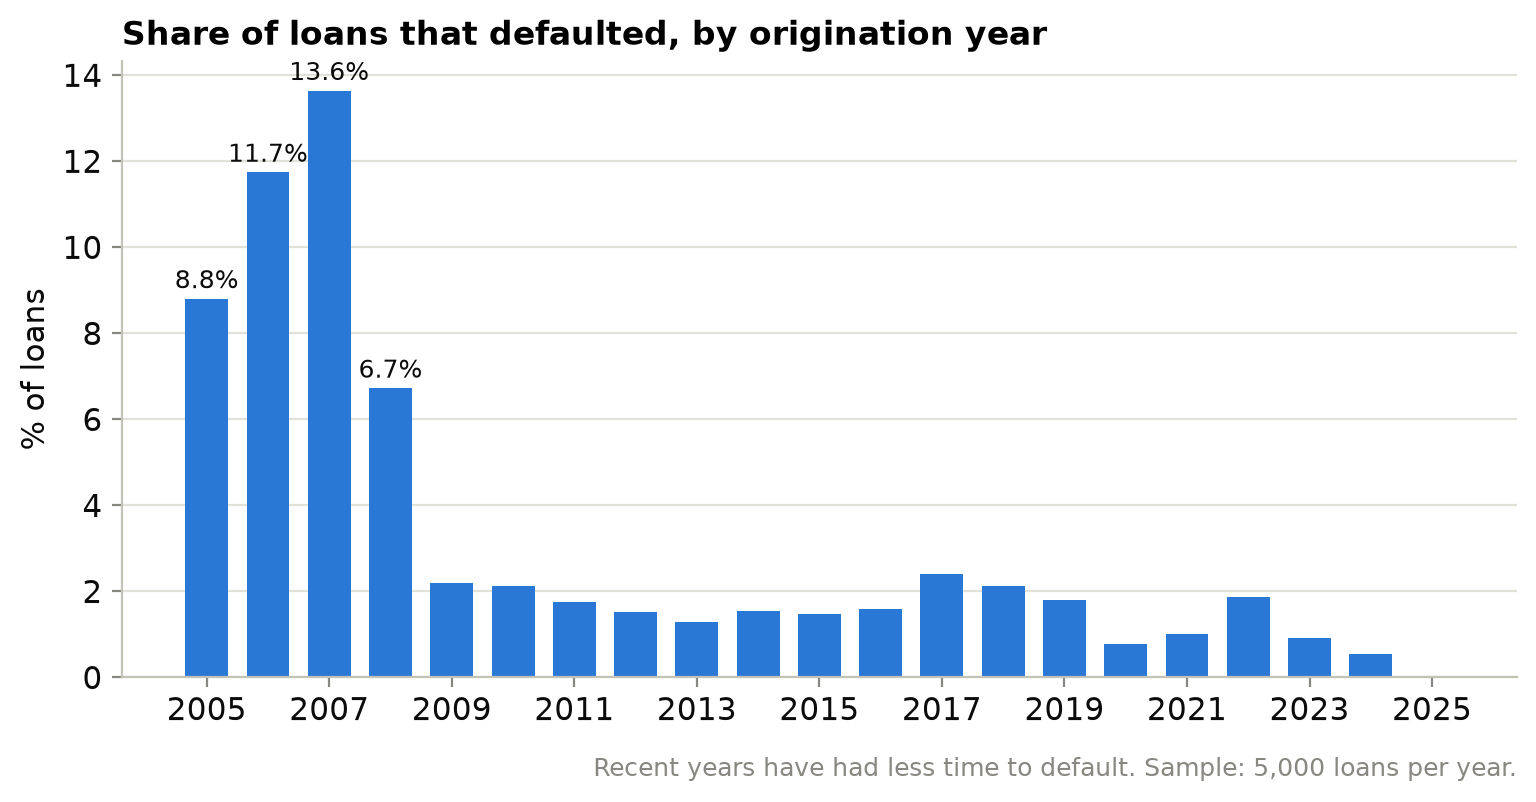
\includegraphics[width=0.85\textwidth]{vintage_defaults.png}
\caption{Share of loans that defaulted by origination year.}
\label{fig:vintage}
\end{figure}

\subsection{Macroeconomic data and scenarios}
Monthly history comes from FRED: the civilian unemployment rate (\texttt{UNRATE}), the FHFA purchase-only house
price index (\texttt{HPIPONM226S}) and the Freddie Mac 30-year fixed mortgage rate (\texttt{MORTGAGE30US}, averaged
to monthly). The October 2025 unemployment rate was never published because of the federal government shutdown;
we fill that single month by linear interpolation.

Forward paths come from the Federal Reserve's 2026 supervisory stress test scenarios (final, February 2026), domestic
variables, which run quarterly from 2026 Q1 to 2029 Q1. The Fed's historical file supplies the 2025 Q4 jump-off
quarter. In the severely adverse scenario unemployment rises from 4.5\% to a peak of 10.0\% in 2027 Q3 and house
prices fall 29.7\% by 2027 Q4. In the baseline unemployment stays between 4.2\% and 4.6\% and house prices are
roughly flat.

\subsection{Benchmark}
For the stress comparison we use the Federal Reserve's \emph{2026 Stress Test Results} (June 2026), Table 9: under
the severely adverse scenario, projected losses on domestic first-lien mortgages across participating banks are
\$22.5 billion, a nine-quarter loss rate of 1.5\% of average balances (2026 Q1--2028 Q1).

\section{Model}

The model has three components, combined month by month in a lifetime loss engine.

\subsection{Probability of default, with prepayment as a competing risk}
In each month $t$ an open loan $i$ either defaults ($D$), prepays ($P$) or keeps paying (the base outcome). We model
the three outcomes jointly with a multinomial logit:
\[
  P(y_{it} = j \mid x_{it}) = \frac{\exp(x_{it}'\beta_j)}{1 + \exp(x_{it}'\beta_D) + \exp(x_{it}'\beta_P)},
  \qquad j \in \{D, P\}.
\]
The probabilities of the three outcomes add to one, so a higher prepayment probability leaves less room for
default, and a loan that prepays leaves the portfolio. The features $x_{it}$ are:
\begin{itemize}
  \item \textbf{Borrower}: FICO score and DTI at origination.
  \item \textbf{Equity}: current LTV, the balance at the start of the month divided by the original property value
        moved with the national house price index, with an extra slope above 100\%.
  \item \textbf{Seasoning}: log of loan age and loan age in years, which together give a hump-shaped age profile.
  \item \textbf{Refinance incentive}: the note rate minus the current 30-year mortgage rate, floored at $-0.5$
        percentage points, plus its positive part (a kink at zero).
  \item \textbf{Macro}: the unemployment rate and year-on-year house price growth.
\end{itemize}
All macro inputs are lagged one month, so the outcome in month $t$ uses only data published by then. The model is
estimated by maximum likelihood on all loan-months through December 2025 (5.6 million observations).

The floor on the refinance incentive came out of the backtest (Section~\ref{sec:backtest}). Below a small negative
incentive, refinancing stops and prepayment is driven by home sales, which do not depend on the interest rate. The
2005--2019 data contain almost no loans with a note rate more than two points below the market rate, while
2023--2025 is full of them. Without the floor the model extrapolates its linear slope and predicts that such loans
almost never prepay.

\subsection{Loss given default}
LGD is a lookup table of realised loss severity (loss divided by balance at default) by current LTV at default, in
buckets with edges at 60, 70, 80, 90, 100 and 120\%. Severities are balance-weighted. Defaulted loans that later
paid off count as zero loss, and loans still unresolved are left out. A bucket with fewer than 30 resolved defaults
uses the overall average. In the projection, current LTV changes every month with the scheduled balance and the
house price path, so falling house prices raise both PD and LGD.

\subsection{Exposure at default}
EAD is the scheduled balance at the start of each month from the level-payment amortization schedule at the note
rate and remaining term. Prepayment does not enter EAD directly; it enters through the probability that the loan is
still open.

\subsection{Macro path: forecast, reversion, long run}
For each scenario the engine builds a monthly path for unemployment, the mortgage rate and house prices. For the
first 24 months it follows the Fed scenario, interpolated from quarterly to monthly. Over the next 12 months each
variable moves linearly to its long-run average, computed over 2000--2025: unemployment 5.6\%, mortgage rate 5.2\%
and house price growth 4.6\% a year. After that the long-run values hold for the rest of each loan's life. House
prices revert in growth terms, so the level never jumps.

The proposal described reverting to long-run \emph{loss rates}. We revert the model's inputs instead, which keeps a
single consistent path for house prices, and therefore for current LTV, PD and LGD.

\subsection{Lifetime expected credit loss}
Let $S_{i,t-1}$ be the probability that loan $i$ is still open at the start of projection month $t$, with
$S_{i,0} = 1$. Then
\[
  \mathrm{ECL}_i = \sum_{t=1}^{T_i} \frac{S_{i,t-1}\;\mathrm{PD}_{it}\;\mathrm{LGD}_{it}\;\mathrm{EAD}_{it}}{(1 + r_i)^t},
  \qquad
  S_{it} = S_{i,t-1}\,\bigl(1 - \mathrm{PD}_{it} - \mathrm{PP}_{it}\bigr),
\]
where $T_i$ is the remaining term, $\mathrm{PP}_{it}$ the prepayment probability and $r_i$ the monthly note rate,
the effective interest rate used for discounting under ASC 326. The portfolio reserve is $\sum_i \mathrm{ECL}_i$,
reported as a percentage of unpaid balance.

The reserve is computed at December 2025, the jump-off date of the 2026 stress test, for every sampled loan that is
open and not yet in default: 34,000 loans with \$8.05 billion of balance. Weighted by balance, the portfolio has an
average FICO of 753, DTI of 36\%, current LTV of 58\% and note rate of 5.24\%. Loans originated in 2020--2025 make up
84\% of the balance, and 44\% of the balance carries a note rate more than one point below the current mortgage rate.

\section{Results}

\subsection{PD model estimates}
Table~\ref{tab:pd} reports the coefficients. The default equation has the expected signs. Fifty points of FICO lower
the odds of default by about 37\%, ten points of DTI raise them by 29\%, and ten points of current LTV raise them by 29\%
up to 100\%, with a flatter slope above. A one-point rise in unemployment raises the monthly odds of default by 11\%.
Borrowers paying above the market rate who have not refinanced default more often (positive coefficient on the
positive part of the incentive), consistent with weaker borrowers being unable to refinance.

In the prepayment equation, the slope on the incentive is 1.37 between $-0.5$ and 0 points and about 0.37 above zero,
so prepayment rises steeply once refinancing becomes worthwhile. Better credit raises prepayment, and high LTV lowers
it, steeply so above 100\%, because borrowers with little equity cannot refinance. The positive coefficient on
unemployment in the prepayment equation is not economically intuitive; it most likely reflects the 2020--2021
refinance boom, which coincided with high unemployment.

\begin{table}[t]
\centering\small
\caption{Multinomial logit estimates, monthly, 2005--2025 (base outcome: keep paying). Standard errors in parentheses.
$^{***}$, $^{**}$, $^{*}$: significant at 1\%, 5\%, 10\%.}
\label{tab:pd}
\begin{tabular}{lrrrr}
\toprule
Variable & \multicolumn{2}{c}{Default} & \multicolumn{2}{c}{Prepayment} \\
\midrule
Constant & $-11.452^{***}$ & $(0.162)$ & $-6.150^{***}$ & $(0.025)$ \\
FICO (per 50 points above 740) & $-0.467^{***}$ & $(0.014)$ & $0.114^{***}$ & $(0.004)$ \\
DTI (per 10 points above 35) & $0.255^{***}$ & $(0.017)$ & $0.006$ & $(0.004)$ \\
Current LTV (per 10 points above 70) & $0.253^{***}$ & $(0.012)$ & $-0.080^{***}$ & $(0.002)$ \\
Current LTV above 100 (per 10 points) & $-0.185^{***}$ & $(0.040)$ & $-0.385^{***}$ & $(0.038)$ \\
log(loan age, months) & $1.005^{***}$ & $(0.056)$ & $0.452^{***}$ & $(0.008)$ \\
Loan age (years) & $-0.153^{***}$ & $(0.017)$ & $-0.137^{***}$ & $(0.003)$ \\
Refinance incentive, floored at $-0.5$ (pct pts) & $-0.094$ & $(0.140)$ & $1.375^{***}$ & $(0.026)$ \\
Positive part of incentive (pct pts) & $0.497^{***}$ & $(0.152)$ & $-1.004^{***}$ & $(0.029)$ \\
Unemployment rate (\%) & $0.108^{***}$ & $(0.010)$ & $0.068^{***}$ & $(0.002)$ \\
House price growth, year on year (\%) & $-0.011^{***}$ & $(0.004)$ & $0.022^{***}$ & $(0.001)$ \\
\bottomrule
\end{tabular}

\end{table}

\subsection{Loss given default}
Table~\ref{tab:lgd} and Figure~\ref{fig:lgd} show the LGD table, estimated from 2,173 resolved defaults. Severity rises
from 7\% for loans below 60\% current LTV, where many defaults cure, to 40\% at 80--100\%. It falls back to about 29\%
above 100\%. The most likely reason is mortgage insurance: loans originated above 80\% LTV carry private mortgage
insurance, which covers part of the loss, and these are the loans most likely to end up above 100\%. The bucket above
120\% has only 22 defaults and uses the overall average.

\begin{table}[t]
\centering\small
\caption{Loss severity by current LTV at default.}
\label{tab:lgd}
\begin{tabular}{lrr}
\toprule
Current LTV (\%) & Resolved defaults & Severity (\%) \\
\midrule
Below 60 & 402 & 7.0 \\
60--70 & 225 & 18.6 \\
70--80 & 341 & 28.8 \\
80--90 & 552 & 39.9 \\
90--100 & 380 & 39.9 \\
100--120 & 251 & 29.0 \\
Above 120 & 22 & 29.5 \\
\bottomrule
\end{tabular}

\end{table}

\begin{figure}[t]
\centering
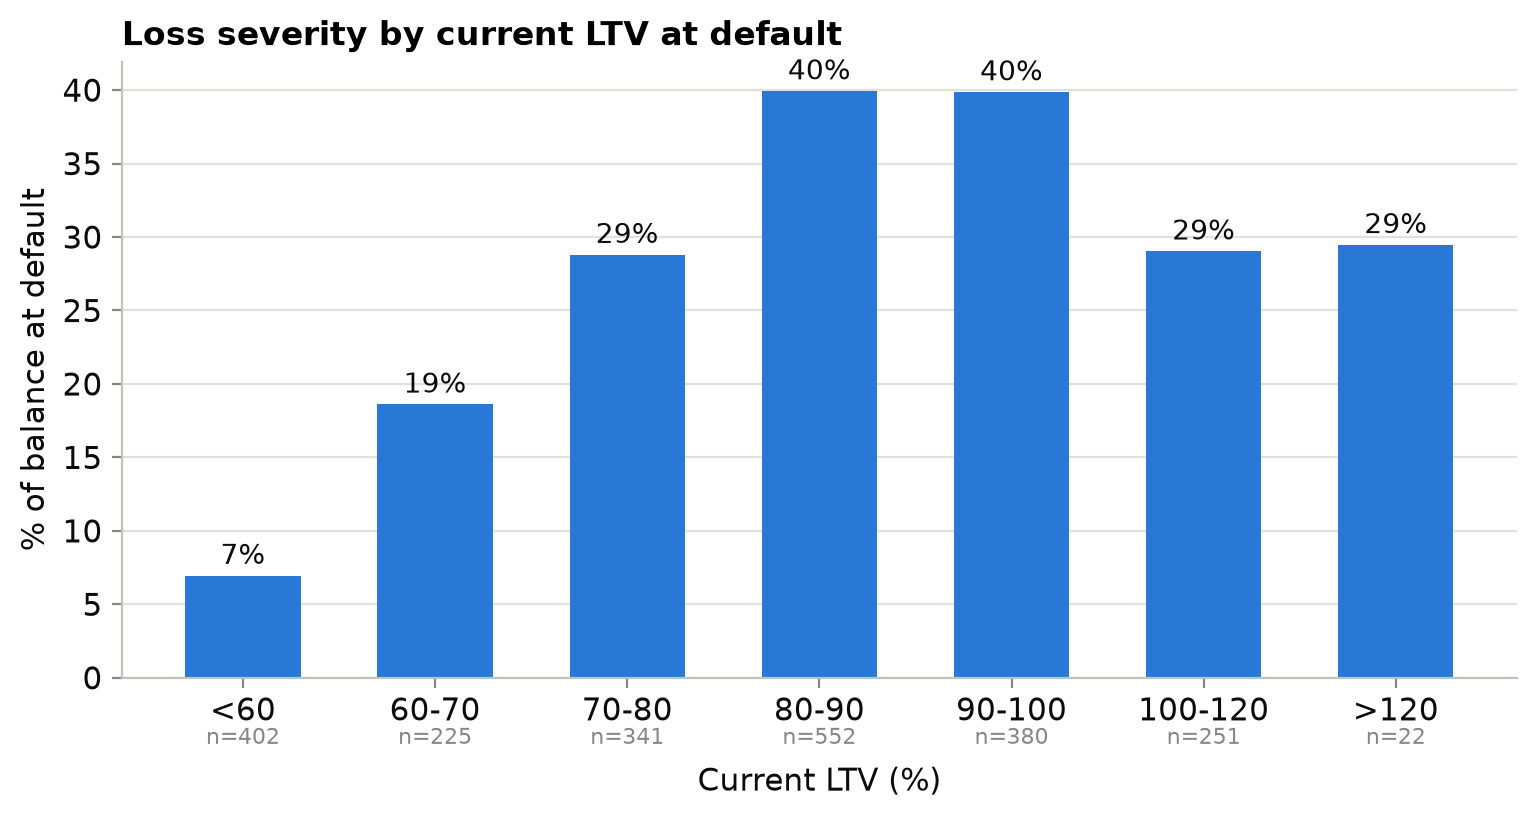
\includegraphics[width=0.75\textwidth]{lgd.png}
\caption{Loss severity by current LTV at default; $n$ is the number of resolved defaults.}
\label{fig:lgd}
\end{figure}

\subsection{Out-of-time backtest}
\label{sec:backtest}
We refit the PD model on 2005--2019 only and predict every loan-month of 2020--2025 (Table~\ref{tab:backtest},
Figure~\ref{fig:backtest}). The model ranks loans reasonably well: out-of-time AUC is 0.74 for default and 0.70 for
prepayment.

\textbf{Prepayment.} The first version of the model, with a linear incentive, predicted 0.17\% a month for 2023
against 0.52\% observed, and 0.39\% for 2025 against 0.73\%. Flooring the incentive at $-0.5$ points brings these to
0.50\% and 0.62\%, and default AUC also rose, from 0.715 to 0.737. It changed the reserve by
less than 0.01 percentage points, because the loans it affects are mostly older low-rate loans with low LTV and little
default risk. The model still under-predicts the 2020--2021 refinance boom (about 2.5\% a month observed against 1.4\%
predicted), which was larger than anything in the training period.

\textbf{Default.} The model expected defaults to spike in 2020, when unemployment reached 14.8\%. Forbearance instead
delayed defaults into 2021, when loans leaving forbearance still 180 days late began to count. From 2022 the model
predicts 0.006--0.014\% a month against an observed 0.025--0.032\%: less than half. This is the main weakness of the
model. A likely cause is that post-COVID defaults come from borrowers who exhausted forbearance and payment deferral,
a process no macro variable in our model captures. Because defaults are under-predicted, the reserve in the next section
is probably understated; a bank in this position would add a qualitative adjustment on top of the modeled number.

\begin{table}[t]
\centering\small
\caption{Out-of-time backtest: model fitted through December 2019, tested on January 2020 to December 2025.}
\label{tab:backtest}
\begin{tabular}{lrr}
\toprule
& Default & Prepayment \\
\midrule
Training loan-months (through 2019-12) & 3,523,421 &  \\
Test loan-months (after 2019-12) & 2,104,268 &  \\
AUC, out of time & 0.737 & 0.697 \\
Actual monthly rate (\%) & 0.038 & 1.259 \\
Predicted monthly rate (\%) & 0.017 & 0.862 \\
\bottomrule
\end{tabular}

\end{table}

\begin{figure}[t]
\centering
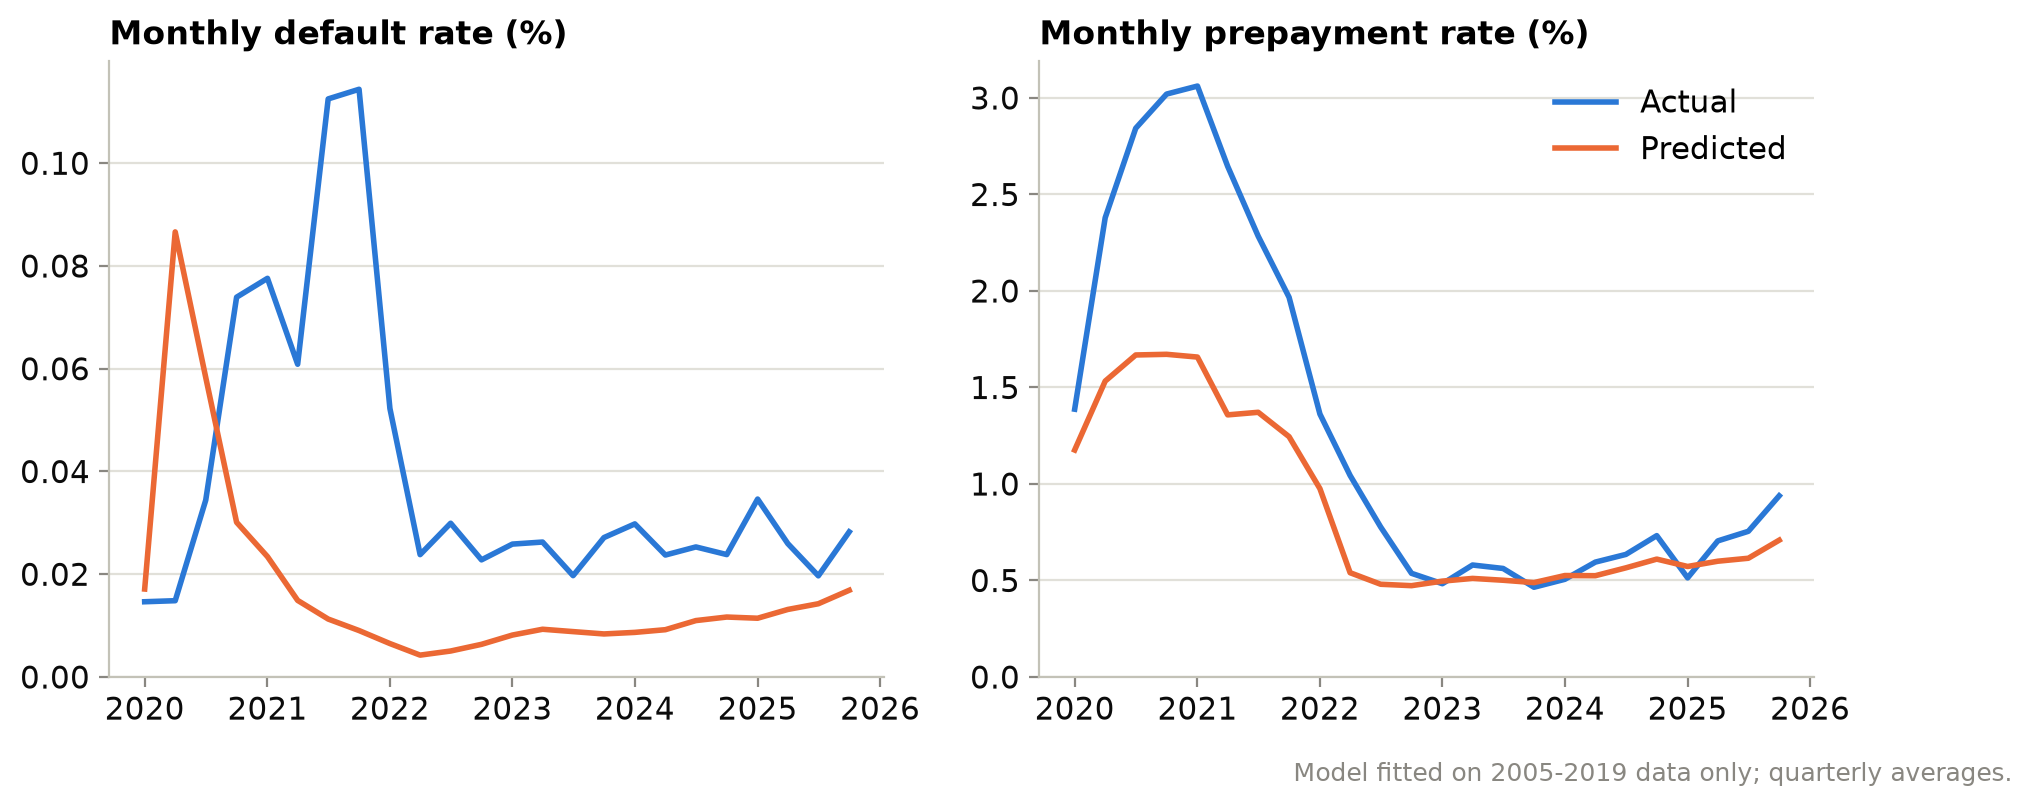
\includegraphics[width=\textwidth]{backtest.png}
\caption{Actual and predicted monthly default and prepayment rates, quarterly averages, 2020--2025.}
\label{fig:backtest}
\end{figure}

\subsection{Allowance by scenario}
Figure~\ref{fig:scenarios} shows the two macro paths and Table~\ref{tab:ecl} the results. The lifetime reserve is
0.44\% of balance (\$35.8 million) under the baseline and 1.54\% (\$123.9 million) under the severely adverse scenario,
about 3.5 times as much. Under stress, the balance expected to default rises from 2.8\% to 6.6\%, and higher current LTV
raises severity at the same time.

Figure~\ref{fig:timing} shows when the losses arrive. Under the severely adverse scenario, monthly expected loss climbs
through 2026--2027 as unemployment rises and house prices fall, peaks at the end of the forecast window, and drops
during the reversion year. Under the baseline it is nearly flat and then rises slightly during reversion, because the
long-run unemployment rate (5.6\%) is above the baseline path (4.2--4.6\%): in this case reversion makes the
reserve \emph{larger}. In both scenarios a little under half of the undiscounted lifetime loss falls in the first nine
quarters.

\begin{figure}[t]
\centering
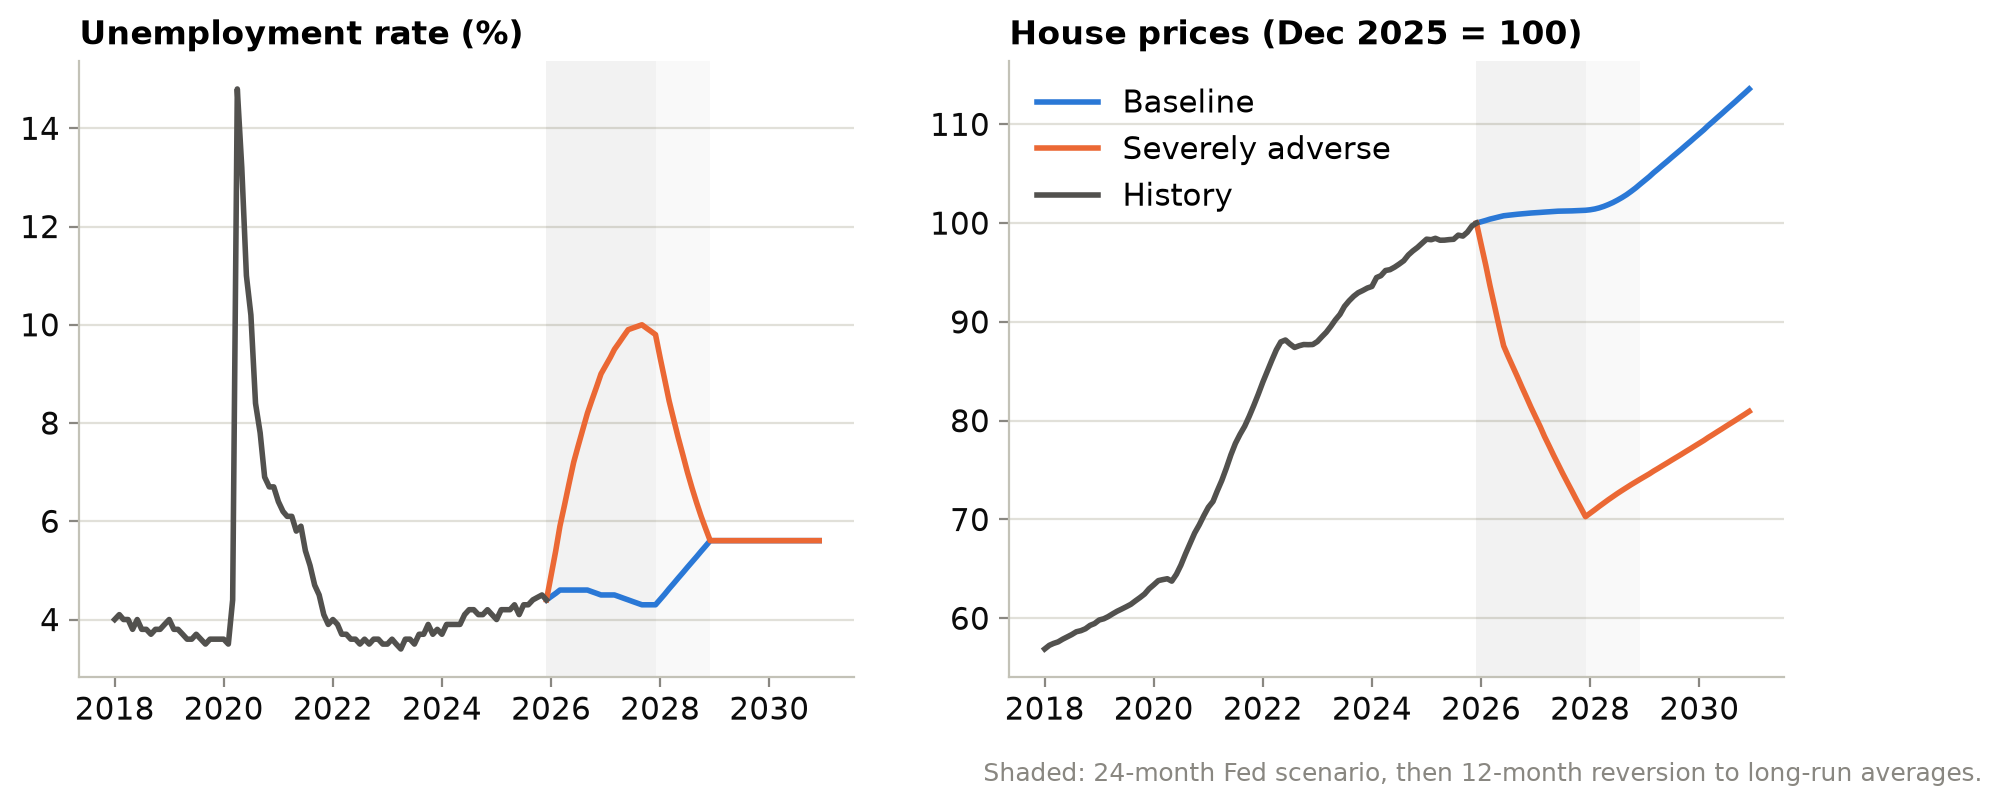
\includegraphics[width=\textwidth]{scenarios.png}
\caption{Unemployment and house prices: history, and the 2026 baseline and severely adverse paths as used by the
engine (24-month scenario, then 12-month reversion to long-run averages).}
\label{fig:scenarios}
\end{figure}

\begin{table}[t]
\centering\small
\caption{Lifetime expected credit loss at December 2025 (24-month forecast, 12-month reversion, discounted at note rates).
Loss and default rates are as a percentage of balance at the reserve date.}
\label{tab:ecl}
\begin{tabular}{lrr}
\toprule
& Baseline & Severely adverse \\
\midrule
Loans open at the reserve date & 34,000 & 34,000 \\
Unpaid balance (\$ billion) & 8.05 & 8.05 \\
Lifetime ECL, discounted (\$ million) & 35.8 & 123.9 \\
Reserve rate (\% of balance) & 0.44 & 1.54 \\
Lifetime loss, undiscounted (\%) & 0.53 & 1.87 \\
Loss in the first 9 quarters (\%) & 0.23 & 0.85 \\
Balance expected to default (\%) & 2.81 & 6.65 \\
\bottomrule
\end{tabular}

\end{table}

\begin{figure}[t]
\centering
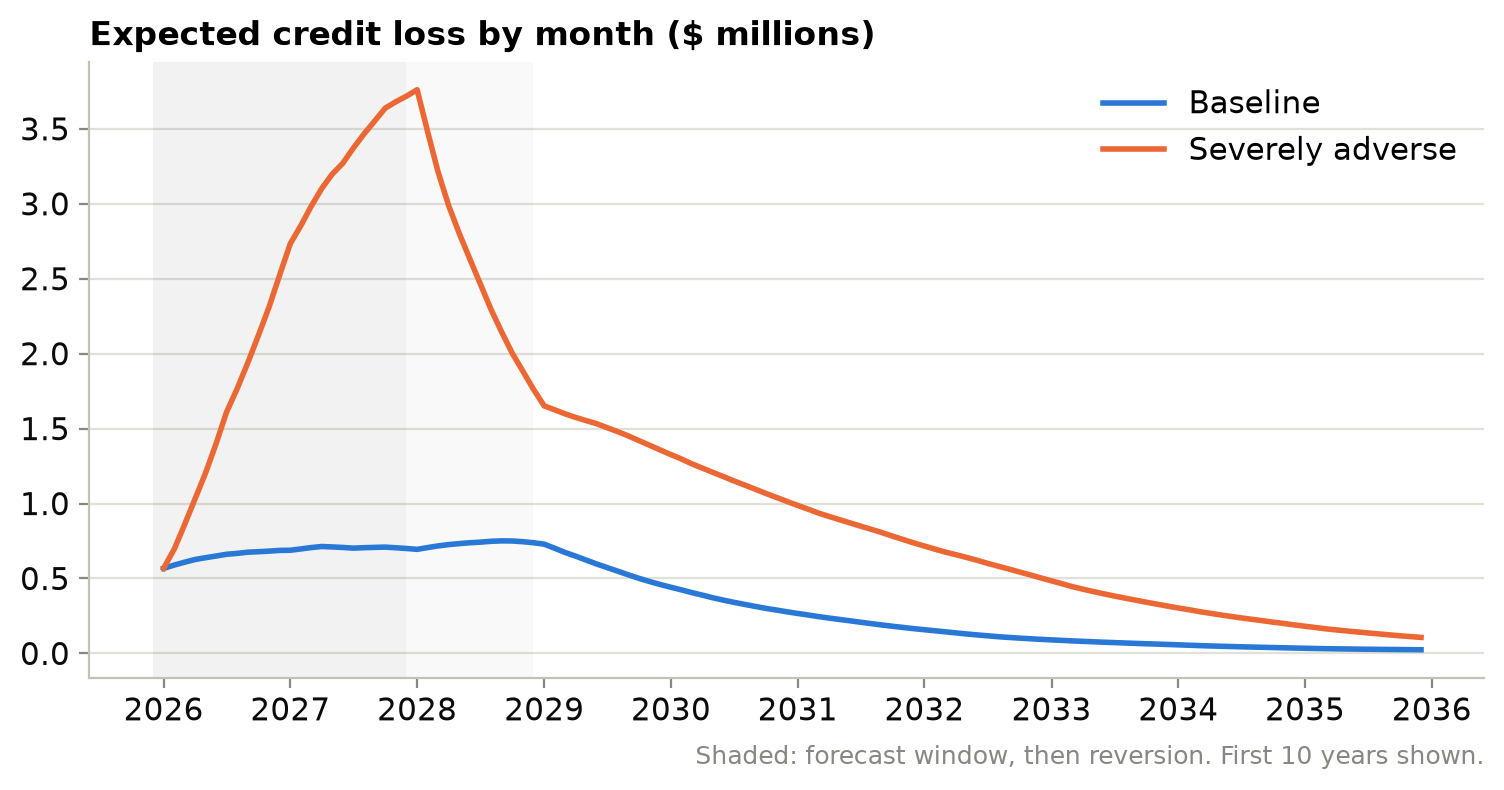
\includegraphics[width=0.85\textwidth]{loss_timing.png}
\caption{Expected credit loss by month, undiscounted, first ten years.}
\label{fig:timing}
\end{figure}

\subsection{Comparison with DFAST}
To compare with the stress test, we follow the severely adverse scenario for its full nine quarters and add up the
expected loss over that period. Our loss rate is 0.85\% of balance, against 1.5\% published by the Federal Reserve
(Figure~\ref{fig:reserve}). A lower number is plausible for three reasons. Freddie Mac loans are conforming loans, with
balance limits and underwriting standards, while bank mortgage books also hold jumbo and non-agency loans. The Fed
divides by average balances over the nine quarters, which shrink as loans pay down, while we divide by the starting
balance. And the default under-prediction in our backtest pushes our number down. The two figures are of the same
order, which suggests the engine responds to the scenario in a sensible way.

\begin{figure}[t]
\centering
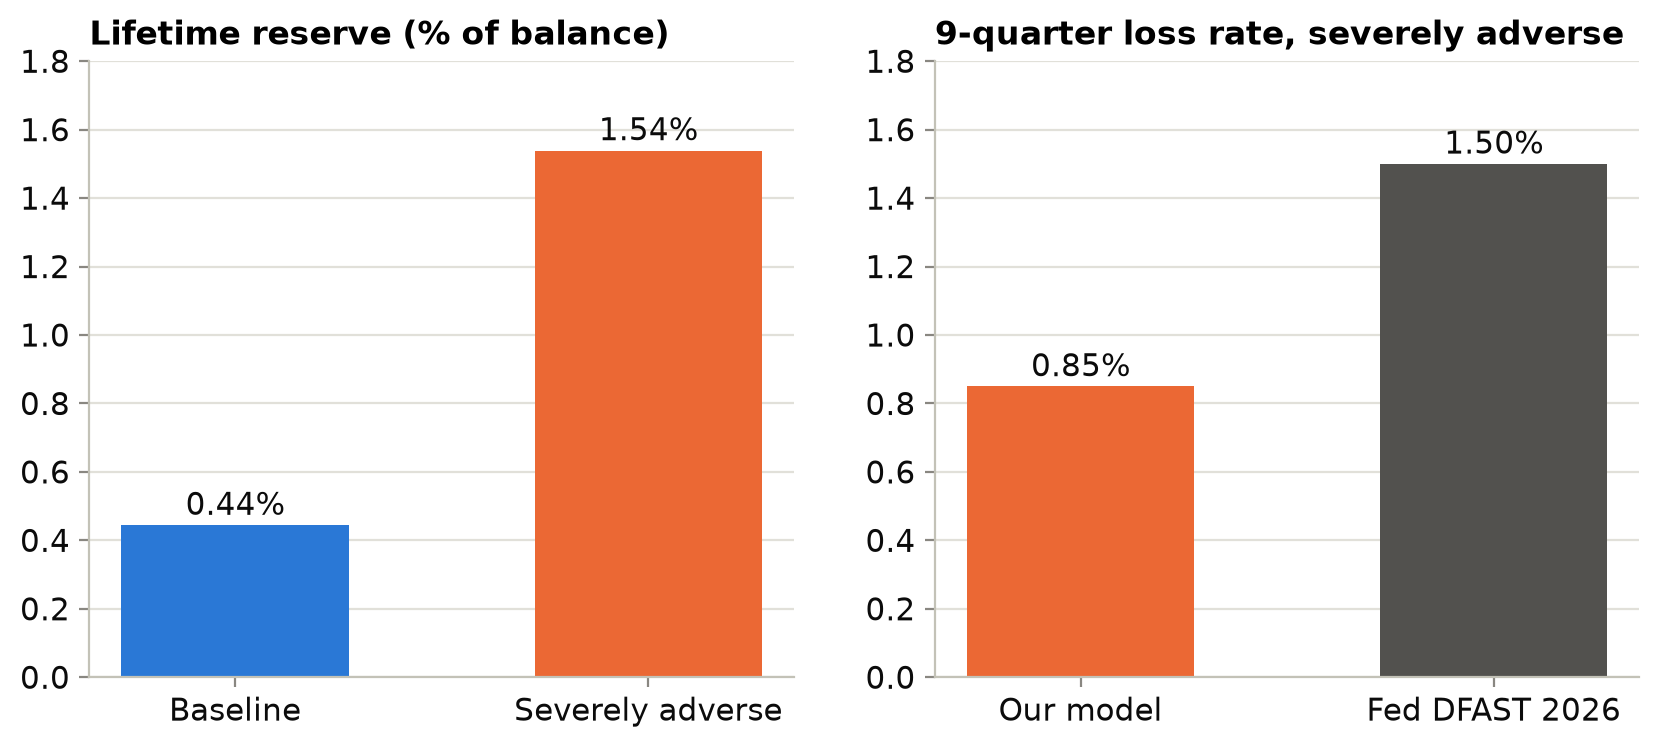
\includegraphics[width=0.85\textwidth]{reserve.png}
\caption{Left: lifetime reserve by scenario. Right: nine-quarter loss rate under the severely adverse scenario, our model
against the Federal Reserve's 2026 DFAST result for domestic first-lien mortgages.}
\label{fig:reserve}
\end{figure}

\subsection{Sensitivity to forecast window and reversion}
Table~\ref{tab:sens} recomputes the reserve for forecast windows of 12, 24 and 36 months and reversion periods of 0, 12
and 24 months. Under the baseline the reserve barely moves (0.40--0.47\%), because the scenario is close to long-run
conditions. Under stress, the window matters a great deal: a 12-month window with immediate reversion gives 0.95\%,
because it cuts the scenario off before unemployment peaks, while a 36-month window with 24-month reversion gives 1.63\%.
Beyond 24 months the scenario is already recovering, so extra months add less. The forecast window is a management
judgment, and in a downturn it can move a mortgage reserve by about 70\%.

\begin{table}[t]
\centering\small
\caption{Reserve rate (\% of balance) by forecast window and reversion period. Base case: 24-month window, 12-month reversion.}
\label{tab:sens}
\begin{tabular}{llrrr}
\toprule
Scenario & Forecast window & No reversion & 12-month reversion & 24-month reversion \\
\midrule
Baseline & 12 months & 0.40 & 0.42 & 0.43 \\
Baseline & 24 months & 0.43 & 0.44 & 0.45 \\
Baseline & 36 months & 0.46 & 0.46 & 0.47 \\
\midrule
Severely adverse & 12 months & 0.95 & 1.20 & 1.36 \\
Severely adverse & 24 months & 1.51 & 1.54 & 1.56 \\
Severely adverse & 36 months & 1.56 & 1.59 & 1.63 \\
\bottomrule
\end{tabular}

\end{table}

\section{Limitations}
\begin{itemize}
  \item \textbf{Default under-prediction after COVID-19.} The model predicts less than half of the defaults observed in
        2022--2025, so the reserve is probably understated.
  \item \textbf{No delinquency status.} The PD model does not know whether a loan is already 30, 60 or 90 days late,
        which is the strongest single predictor of default. Using it would require projecting delinquency transitions.
  \item \textbf{National macro variables only.} Regional house prices and unemployment would capture local downturns.
  \item \textbf{LGD depends on the scenario only through house prices.} It ignores liquidation timelines and the
        mortgage insurance pattern seen above 100\% LTV.
  \item \textbf{Sample composition.} Each origination year contributes 5,000 loans regardless of how many Freddie Mac
        actually bought that year, and conforming fixed-rate loans are not representative of a whole bank mortgage book.
\end{itemize}

\section{Changes from the proposal}
\begin{itemize}
  \item Reversion is applied to the macro inputs rather than to long-run loss rates (Section 3.4).
  \item The refinance incentive is floored at $-0.5$ points after the backtest showed the linear version under-predicted
        prepayment by more than half in 2023--2025.
  \item Forbearance months are excluded from the default definition.
  \item The optional gradient boosting model with SHAP explanations was not pursued; we kept the transparent
        multinomial logit.
\end{itemize}

\section{Conclusion}
CECL turns the allowance into a forecast, and our results show how much that forecast depends on choices outside the
credit model itself. Moving from the baseline to the severely adverse scenario multiplies the reserve by about 3.5,
and under stress the forecast window alone moves it between 0.95\% and 1.63\%. Treating prepayment as a competing risk
is necessary, and how prepayment is extrapolated matters: a linear refinance incentive fitted on 2005--2019 badly
under-predicts prepayment in today's high-rate environment. The remaining weakness, under-predicted defaults after
COVID-19, is the kind of model limitation that CECL practice addresses with a documented qualitative adjustment.

\section*{References}
\begin{itemize}
  \item Financial Accounting Standards Board (2016). \emph{Accounting Standards Update 2016-13, Financial Instruments---Credit
        Losses (Topic 326): Measurement of Credit Losses on Financial Instruments.}
  \item Freddie Mac. \emph{Single-Family Loan-Level Dataset} and \emph{General User Guide}. Sample files, release with
        performance through June 2026.
  \item Board of Governors of the Federal Reserve System (2026). \emph{2026 Stress Test Scenarios} (February 2026), with
        the supervisory baseline, severely adverse and historic domestic variable files.
  \item Board of Governors of the Federal Reserve System (2026). \emph{2026 Federal Reserve Stress Test Results} (June 2026).
  \item Federal Reserve Bank of St.\ Louis. FRED series UNRATE, HPIPONM226S and MORTGAGE30US, \url{https://fred.stlouisfed.org}.
\end{itemize}

\appendix
\section{Code and reproduction}
The submission zip contains the Python package and all result tables. The Freddie Mac data cannot be redistributed under
its licence, so it is not included; \texttt{README.md} explains how to download each input.

\begin{tabular}{@{}lp{0.6\textwidth}@{}}
\texttt{config/default.yaml} & every setting: vintages, sample size, default rule, reserve date, windows \\
\texttt{src/cecl/freddie.py} & readers for the raw Freddie Mac files \\
\texttt{src/cecl/macro.py} & FRED download, Fed scenario loader, forecast--reversion--long-run path \\
\texttt{src/cecl/panel.py} & loan-month panel with outcomes; defaults table with realised losses \\
\texttt{src/cecl/features.py} & design matrix shared by estimation and projection \\
\texttt{src/cecl/models.py} & competing-risk logit, LGD table, amortization \\
\texttt{src/cecl/engine.py} & lifetime ECL engine \\
\texttt{src/cecl/figures.py} & figures in this report \\
\texttt{src/cecl/report\_tables.py} & tables in this report \\
\texttt{tests/} & unit tests, including a closed-form check of the ECL engine \\
\texttt{outputs/} & result tables (CSV) behind every number in this report \\
\end{tabular}

To reproduce, with Python 3.11 and the data in place:
\begin{verbatim}
make setup     # virtual environment and dependencies
make macro     # download FRED history
make all       # build panel, fit, ECL, backtest, sensitivity (about a minute)
make figures   # figures and tables for this report
make report    # this PDF
\end{verbatim}

\end{document}
